%%
%% 研究報告用スイッチ
%% [techrep]
%%
%% 欧文表記無しのスイッチ(etitle,jkeyword,eabstract,ekeywordは任意)
%% [noauthor]
%%

\documentclass[submit,techrep]{ipsj}
%\documentclass[submit,techrep,noauthor]{ipsj}



\usepackage[dvipdfmx]{graphicx}
\usepackage{latexsym}

\def\Underline{\setbox0\hbox\bgroup\let\\\endUnderline}
\def\endUnderline{\vphantom{y}\egroup\smash{\underline{\box0}}\\}
\def\|{\verb|}

\setcounter{巻数}{53}%vol53=2012
\setcounter{号数}{10}
\setcounter{page}{1}


\begin{document}


\title{データベース及び演習\\
(2023年6月12日)}

\etitle{Database and Exercises \\ (version 2012/10/12)}

\affiliate{IPSJ}{情報処理学会\\
IPSJ, Chiyoda, Tokyo 101--0062, Japan}


\paffiliate{JU}{情報処理大学\\
Johoshori Uniersity}

\author{水谷祐生}{Yusei Mizutani}{IPSJ}[joho.taro@ipsj.or.jp]

\begin{abstract}
本稿は,情報処理学会論文誌ジャーナルに投稿する原稿を執筆する際,および論
文採択後に最終原稿を準備する際の注意点等をまとめたものである.大きく分け
ると,論文投稿の流れと,\LaTeX と専用のスタイルファイルを用いた場合の論
文フォーマットに関する指針,および論文の内容に関してするべきこと,するべ
きでないことをまとめたべからずチェックリストからなる.本稿自体も \LaTeX 
と専用のスタイルファイルを用いて執筆されているため,論文執筆の際に参考に
なれば幸いである.
\end{abstract}

%
%\begin{jkeyword}
%情報処理学会論文誌ジャーナル,\LaTeX,スタイルファイル,べからず集
%\end{jkeyword}
%
%\begin{eabstract}
%This document is a guide to prepare a draft for submitting to IPSJ
%Journal, and the final camera-ready manuscript of a paper to appear in
%IPSJ Journal, using {\LaTeX} and special style files.  Since this
%document itself is produced with the style files, it will help you to
%refer its source file which is distributed with the style files.
%\end{eabstract}
%
%\begin{ekeyword}
%IPSJ Journal, \LaTeX, style files, ``Dos and Dont's'' list
%\end{ekeyword}

\maketitle

%1
\section{機能概要}

教科書9章、10章に記されているサンプルコードにはユーザーからメールアドレス、パスワード、出身地、生年月日を受け付け、メールを用いて認証を行う会員登録機能と、会員登録を行なった後に専用ページに遷移するためのログイン機能、認証を行なった後、専用ページから退出するログアウト機能、認証されたユーザーを一覧することのできる管理者機能が実装されている.

また、全体の操作の流れは、ログイン画面から新規登録画面に遷移し、新規登録画面でメールアドレス、パスワード、出身地、生年月日を受け付ける.  その後、入力したメールアドレスで登録確認を行うとログイン者専用画面に遷移する流れとなっている.

\section{利用技術}
\subsection{PHP}
PHPとは「ピー・エイチ・ピー」と読み、Personal Home Pageがその由来である.

主に、Webで利用されるHTML形式のようなハイパーテキストを閲覧者の操作によって動的な画面を作ることを得意としている. 

PHPの特徴として誰でも無償で利用できるオープンソースのサーバサイド・スクリプト言語であることが挙げられる.さらに、無償で利用できるからと言ってメンテナンスがされていないなどはなく、マニュアル、バグ修正なども十分に行われているため、安心して利用できる. 

また、多様なDB、ライブラリへの対応、デバッグのしやすさ、その習得のしやすさなどからプログラミング言語を初めて学ぶ人たちにも扱いやすい言語となっている.

\subsection{MariaDB/MySQL}
MySQLとはオープンソースソフトウェアのRDBMD(relational database management system)であり、現在はOracle社が管理している.

一方、MariaDBとは、MySQLから派生したRDBMDであり、MySQLのソースコードをベースにして、新機能追加やソースコードの改善が組み込まれている.

両者共に互換性があり、同じSQL文を用いてデータベース操作を行なっているが、もちろん違いもある.

両者の違いとして、無償で全ての機能が使えるかどうかである.MariaDBは完全なGPLライセンスでその全ての機能が使用可能である。一方で、MySQLは特別な機能は有料のライセンスに含まれるとする、デュアルライセンス方式を採用している.

\subsection{CSS}
CSSとは(Cascading Style Sheets)は、「シー・エス・エス」と読み、Webページのデザインやレイアウトを制御する言語である. 主にHTMLやXHTMLなどで作成されるウェブページにスタイルを適用したい場合に用いられている.

CSSを使用しなくとも、HTMLには\<center\>や\<font\>タグなどの装飾目的の要素や属性が存在しているため、HTMLだけでウェブページの見栄えを制御することもできなくはない.しかし、HTMLは情報構造を定義するための言語であり、見栄えの制御のために本来の役割とは違った使い方をすると、 文書の情報構造がでたらめになってまうため、スタイリングにHTMLを用いるべきではないとされている.

そこで HTMLでは文書構造のみを定義して、 スタイルについてはCSSow用いたスタイリングシートで指定することが推奨されている.そうすることで他の閲覧環境に依存せず、HTMLを本来の役割で使用することが可能になった.





\subsection{Smarty}
Smartyとは、2000年代前半にリリースされたスクリプト言語であるPHPのテンプレートエンジンである.

テンプレートエンジンとは「機能を記述する内容(PHP)」と「画面の表示内容(HTML&CSSなど)」を分けて管理できるツールである.

単純なページや数ページ程度ではテンプレートエンジンの恩恵を感じることができないが、PCとスマートフォンで別々のレイアウトを用意したい時や、膨大なページ数を用意する場合、その便利さを感じることができる.

従来は開発の際、HTMLの中にPHPを埋め込む手法を取っていた.しかし、PHPとHTMLが混在したファイルは、2つのルールが一緒に書かれているので読み取りにくい点が難点であった.両方のプログラミング言語が混在して1つのファイルに書かれている場合、修正にはページ数が多いほど膨大な時間がかかり、保守やメンテナンスがしづらいといった問題があった.

そこで、Smatryを用いることで、機能と表示内容の分離、つまりHTMLとPHPを別のファイルで記述することができる.こうすることで、プログラマーとデザイン担当の作業ファイルを完全に分割することができるため、開発を効率的に行うことが可能になった.

\subsection{HTTP}
HTTP(HTTP: HyperText Transfer Protocol) とは、Web情報をやりとりするプロトコルの一種であり、ホームページやブログを閲覧する際、HTTPを用いてサーバとクライアント間でやり取りが行われている.

特徴として、動作がとてもシンプルであることが挙げられる.情報のやり取りは常に、クライアントが要求を出し、サーバが応答を返します。HTTPは1リクエスト1レスポンスを返すルールがあるため、どちらかが多くなることはあり得ない.また、あるリクエストに対するレスポンスは必ず同じものになる特徴がある.

このように、HTTPは完結で分かりやすい特性を持つことから、WebサーバとWebブラウザ間のやり取り以外に、スマホやアプリからのサーバ機能呼び出しや、サーバ間のサービス呼び出しなどに幅広く使われている.

\subsection{SMTP/IMAP/POP}
SMTPとはシンプル・メール・トランスファー・プロトコルと読み、Simple Mail Transfer Protocolがその由来である.主に、インターネットなどのTCP / IPネットワークで用いられており、メールを送信するための通信プロトコルの一つである.

一方でPOPとはポスト・オフィス・プロトコルと読み、Post Office Protocolがその由来である.こちらもSMTP同様にインターネットなどのTCP / IPネットワークで用いられているプロトコルであるが、SMTPと異なり、メールを受信するための通信プロトコルである.


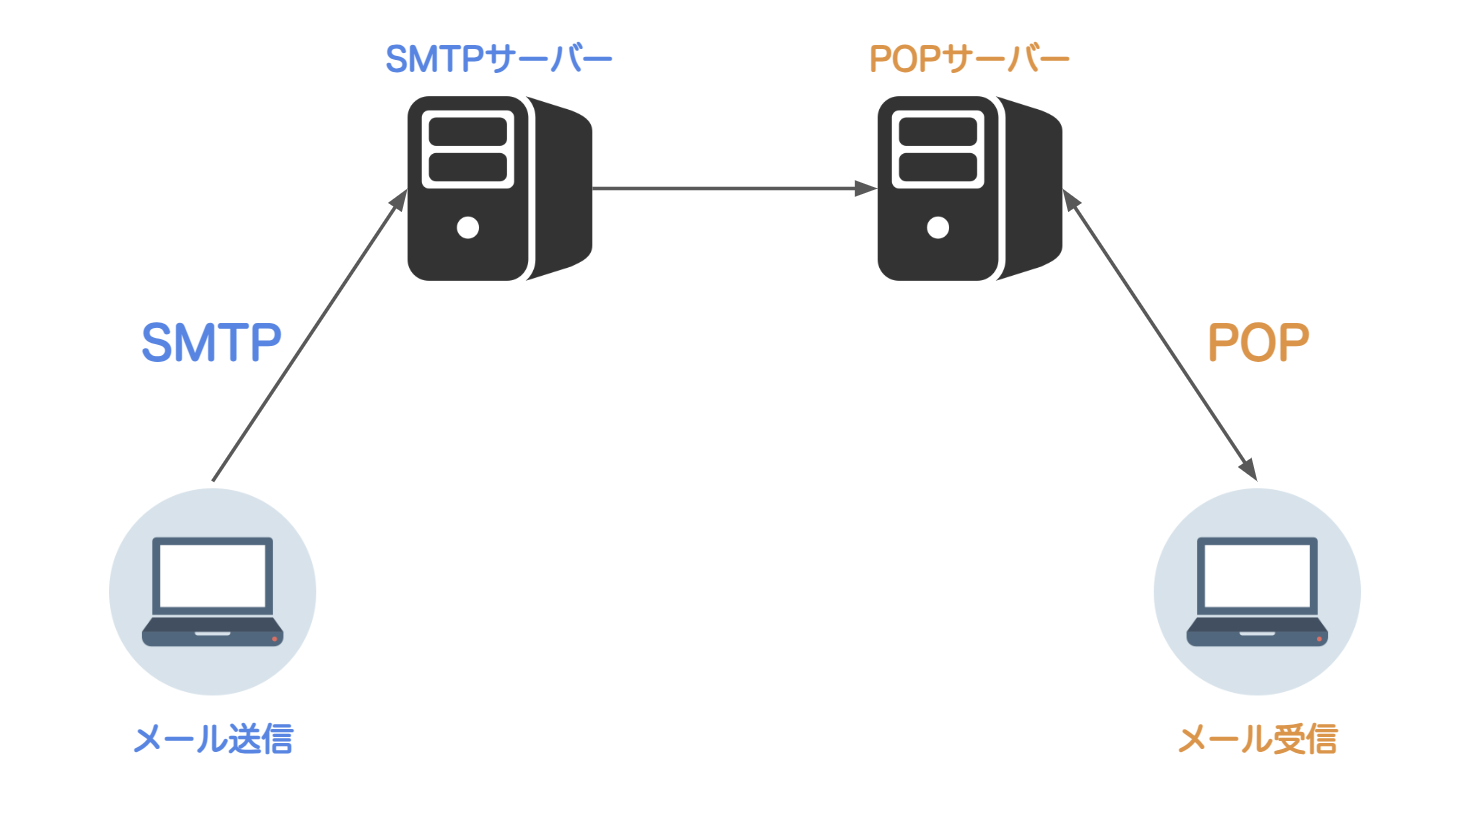
\includegraphics[width=8cm]{./images/mail.jpg}

メール送受信の仕組みとしては、上記の画像のようになっており、

\begin{enumerate}
  \item SMTPでメールをサーバーに送信する
  \item SMTPサーバーからPOPサーバーに受信したメールの内容を送信する
  \item  POPサーバーから受け取る側のPCにメールの内容を送信する
  \end{enumerate}

といった流れになっている.
\section{システム設計}
\subsection{システム概要}



情報処理学会論文誌ジャーナルの \LaTeX スタイルファイルを含む論文執筆キッ
トは
\begin{quote}
\small
\|http://www.ipsj.or.jp/jip/submit/style.html|
\end{quote}
からダウンロードすることができる.論文執筆キットは以下のファイルを含んで
いる.
\begin{enumerate}
\item \|ipsj.cls      |: 最終原稿用スタイルファイル
\item \|ipsjdraft.sty |: 投稿用スタイル(査読用)
\item \|ipsjpref.sty  |: 序文用スタイル
\item \|jsample.tex   |: 本稿のソースファイル
\item \|esample.tex   |: 英文サンプルのソースファイル
\item \|ipsjsort.bst  |: jBibTEX スタイル(著者名順)
\item \|ipsjunsrt.bst |: jBibTEX スタイル(出現順)
\item \|bibsample.bib |: 文献リストのサンプル
\item \|ebibsample.bib|: 英文文献リストのサンプル
\end{enumerate}
キットはUnix用,Windows (DOS)用,Macintosh用などが用意されており,著者の
作業環境に応じたものを選択できるようになっている.また,実行環境としては 
\LaTeXe を前提としているので,準備されたい.

Microsoft Wordに関しては,投稿されたフォーマットを基に,業者が \LaTeX に
変換して組版を行うので,あくまでも参考としてしか使わないことを承知して頂
きたい.

%2.2
\subsection{最終原稿の作成と投稿}

本稿に従って用意した投稿用原稿の \LaTeX ソースからpdfファイルを作成し,
Adobeのpdf readerで読めることを確認した後,
\begin{quote}
\small
\|https://www.ipsj.or.jp/prms/author_pre_submit.do|
\end{quote}
のPRMS (Paper Review Management System)にメールアドレスを登録し,送られ
たきたメールに従って,指定されたURLから投稿する.投稿の流れについては,
\begin{quote}
\small
\|http://www.ipsj.or.jp/journal/submit/manual/|
\|manual_j_for_Author.pdf|
\end{quote}
を参照されたい.

なお,情報処理学会論文誌ジャーナルでは,論文の著者が査読者の名前を知るこ
とがないだけなく,査読者も著者の名前を知らないダブルブラインドの査読を取
り入れている.このため,投稿版では,原稿に著者名とその所属は表示しないよ
うにする必要がある.

%2.3
\subsection{最終原稿の作成とファイルの送付}

投稿した論文の採録が決定したら,査読者からのコメントなどにしたがって原稿
を修正し,著者紹介など投稿時になかった項目があれば追加する.また図表など
のレイアウトも最終的なものとする.なお後の校正の手間を最小にするために,
この段階で記述の誤りなどを完全に除去するように綿密にチェックして頂きたい.

最終版では,著者名およびその所属を表示すると同時に,学会より指示された巻
数,号数,先頭ページ番号,受付/採録年月日(年は西暦)を記述する.なお学
会からの指示がない項目に関しては,記述しなくてよい.

学会へは{\bf \LaTeX ファイル(をまとめたもの)とハードコピーの双方を}送
付する.送付するファイル群の標準的な構成は \|.tex| と \|.bbl| であり,こ
の他にPostScriptファイルや特別なスタイルファイルがあれば付加する.なお 
\|.tex| は印刷業者が修正することがあるので,{必ず一つのファイルにする}.
また必要なファイルが全てそろっていること,特に特別なスタイルファイルに洩
れがないことを,注意深く確認して頂きたい.

ファイルの送付方法などについては,採録通知とともに学会事務局から送られる
指示に従う.

%2.4
\subsection{著者校正・組版・出版}

学会では用語や用字を一定の基準に従って修正することがある.また \LaTeX の
実行環境の差異などによって著者が作成したハードコピーと実際の組版結果が微
妙に異なることがある.これらの修正や差異が問題ないかを最終的に確認するた
めに,著者にゲラ刷りが送られるので,もし問題があれば朱書によって指摘して
返送する.なお{\bf この段階での記述誤りの修正は原則として認められない}の
で,原稿送付時に細心の注意を払っていただきたい.

その後,著者の校正に基づき最終的な組版を行ない,オンライン出版する.



%3
\section{論文フォーマットの指針}
\label{sec:format}

以下,情報処理学会論文誌ジャーナル用スタイルファイルを用いた論文フォーマッ
トの指針について述べるので,これに従って原稿を用意頂きたい.\LaTeX を用
いた一般的な文章作成技術については,\cite{okumura, companion} 等を参考に
されたい.

%4
\section{論文の構成}
\label{config}

ファイルは次のようになる.下線部は投稿時に省略可能なもの.またトランザク
ション特有コマンドについては \ref{sig}~節を参照されたい.

\noindent
\|\documentclass[submit]{ipsj}|または\\
\|\documentclass[submit,draft]{ipsj}|\footnote{{\tt [draft]}は投稿用,
スタイルオプションは\ref{option}節参照.}
\\
\quad 必要ならばオプションのスタイルを追加\\
\Underline{\|\setcounter{|{\bf 巻数}\|}{<巻数>}|}\\
\Underline{\|\setcounter{|{\bf 号数}\|}{<号数>}|}\\
\Underline{\|\setcounter{|{\bf page}\|}{<先頭ページ>}|}\\
\Underline{\|\|{\bf 受付}\|{<年>}{<月>}{<日>}|}\\
\Underline{\|\|{\bf 採録}\|{<年>}{<月>}{<日>}|}\\
\quad 必要ならばユーザのマクロをここに記述\\
\|\begin{document}|\\
\|\title{表題(和文)}|\\
\|\etitle{表題(英文)}|\\
\Underline{\|\affiliate{所属ラベル}{<和文所属>\\<英文所属>}|}\\
\quad 必要ならば \|\paffiliate| により現在の所属を宣言する\\
\Underline{\|\paffiliate{現所属ラベル}{<和現所属>\\<英現所属>}|}\\\\
\Underline{\|\author{情報 太郎}{Taro Joho}|}\\
\Underline{\|          {<所属ラベル>}[E-mail]|}\\
\Underline{\|\author{処理 花子}{Hanako Shori}|}\\
\Underline{\|          {<所属ラベル2,現所属ラベル3>}|}\\\\
\|\begin{abstract}|\\
\|<概要(和文)>|\\
\|\end{abstract}|\\
\|\begin{jkeyword}|\\
\|<キーワード>|\\
\|\end{jkeyword}|\\
\|\begin{eabstract}|\\
\|<概要(英文)>|\\
\|\end{eabstract}|
\|\begin{ekeyword}|\\
\|<KeyWords>|\\
\|\end{ekeyword}|\\
\|\maketitle|\\
\|\section{|第1節の表題\|}|\\
\dots\dots\dots\dots\dots\\
\quad \|<本文>|\\
\dots\dots\dots\dots\dots\\
謝辞がある場合は\\
\|\begin{acknowledgment}|\\
\|\end{acknowledgment}|\\\\
\|\begin{thebibliography}{99}%9 or 99|\\
\|\bibitem{1}|\\
\|\bibitem{2}|\\
\|\end{thebibliography}|\\\\
付録がある場合は\\
\|\appendix|\\
\|\section{|付録1節の表題\|}|\\\\
\Underline{\|\begin{biography}|}\\
\Underline{\|\profile{<X>}{<苗字 名前>}{<プロフィール文章>}|}\\
\Underline{\|\end{biography}|}\\
\|\end{document}|


%4.1
\subsection{オプション・スタイル}

\label{option} \|\documentclass{ipsj}|のオプション\footnote{研究会用のオ
プションは \ref{sig}~節で説明する.}として,以下のものを用意してある.
{\bf 何も定義しなければ和文論文用の標準スタイル}となるが,今回,組版の際
に和文論文のタイトル,和文論文種別に「{\bf 太ミン}」「{\bf 太ゴ}」のフォ
ントを使用しているため,\TeX 標準フォントに置き換える \|submit| というオ
プションを用意した.

\begin{enumerate}
\item\|submit         | フォント置換用
\item\|draft          | 投稿用
\item\|invited        | 招待論文
\item\|sigrecommended | 推薦論文
\item\|technote       | テクニカルノート用
\item\|preface        | 序文用
\item\|JIP            | 英文用
\end{enumerate}
これらのオプションは任意の組合せで使用が可能である.

\|\documentclass[submit,draft]{ipsj}|とすれば,
投稿用のスタイルとなる.

なお,\|\usepackage| で補助的なスタイルファイルを指定した場合には,最終
原稿用のファイル群に必ずスタイルファイルを含める.ただし,\LaTeXe の標準
配布に含まれているもの(たとえば \|graphicx|)については同封の必要はない.

スタイルファイルによっては論文誌スタイルと矛盾するようなものもあるので,
注意して使用して頂きたい.

%4.2
\subsection{表題・著者名等}

表題,著者名とその所属,および概要を前述のコマンドや環境により{\bf 和文と
英文の双方について}定義した後,\|\maketitle| によって出力する.

%4.2.1
\subsubsection{表題} 

表題は,\|\title| および \|\etitle| で定義した表題はセンタリングされる.
文字数の多いものについては,適宜 \|\\| を挿入して改行する.

%4.2.2
\subsubsection{著者名・所属} 

各著者の所属を第一著者から順に \|\affiliate| を用いてラベル(第1引数)を
付けながら定義すると,脚注に番号を付けて所属が出力される.なお,複数の著
者が同じ所属である場合には,一度定義するだけで良い.


\subsubsection{概要} 

%4.2.4
\subsubsection{キーワード} 

%4.3
\subsection{本文}

%4.3.1
\subsubsection{見出し}

節や小節の見出しには \|\section|, \|\subsection|, \|\subsubsection|,
\|\paragraph| といったコマンドを使用する.

\<「定義」,「定理」などについては,\|\newtheorem|で適宜環境を宣言し,そ
の環境を用いて記述する.

%4.3.2
\subsubsection{行送り}

2段組を採用しており,左右の段で行の基準線の位置が一致することを原則とし
ている.また,節見出しなど,行の間隔を他よりたくさんとった方が読みやすい
場所では,この原則を守るようにスタイルファイルが自動的にスペースを挿入す
る.したがって本文中では \|\vspace| や \|\vskip| を用いたスペースの調整
を行なわないようにすること.

%4.3.3
\subsubsection{フォントサイズ}

フォントサイズは,スタイルファイルによって自動的に設定されるため,基本的
には著者が自分でフォントサイズを変更する必要はない.

%4.3.4
\subsubsection{句読点}

句点には全角の「.」,読点には全角の「,」を用いる.ただし英文中や数式中
で「.」や「,」を使う場合には,半角文字を使う.「。」や「、」は使わない.

%4.3.5
\subsubsection{全角文字と半角文字}

全角文字と半角文字の両方にある文字は次のように使い分ける.

\begin{enumerate}
\item 括弧は全角の「(」と「)」を用いる.但し,英文の概要,図表見出し,
書誌データでは半角の「(」と「)」を用いる.

\item 英数字,空白,記号類は半角文字を用いる.ただし,句読点に関しては,
前項で述べたような例外がある.

\item カタカナは全角文字を用いる.

\item 引用符では開きと閉じを区別する.
開きには \|``| を用い,閉じには\|''| を用いる.
\end{enumerate}

%4.3.6
\subsubsection{箇条書}

箇条書に関する形式を特に定めていない.場合に応じて標準的な \|enumerate|,
\|itemize|, \|description| の環境を用いてよい.


%4.3.7
\subsubsection{脚注}

脚注は \|\footnote| コマンドを使って書くと,ページ単位に\footnote{脚注の
例.}や\footnote{二つめの脚注.}のような参照記号とともに脚注が生成される.
なお,ページ内に複数の脚注がある場合,参照記号は \LaTeX を2回実行しない
と正しくならないことに注意されたい.

また場合によっては,脚注をつけた位置と脚注本体とを別の段に置く方がよいこ
ともある.この場合には,\|\footnotemark| コマンドや \|\footnotetext| コ
マンドを使って対処していただきたい.

なお,脚注番号は論文内で通し番号で出力される.

%4.3.8
\subsubsection{OverfullとUnderfull}

組版時にはoverfullを起こさないことを原則としている.従って,まず提出する
ソースが著者の環境でoverfullを起こさないように,文章を工夫するなどの最善
の努力を払っていただきたい.但し,\|flushleft| 環境,\|\\|,
\|\linebreak| などによる両端揃えをしない形でのoverfullの回避は,できるだ
け避けていただきたい.また著者の執筆時点では発生しないoverfullが,組版時
の環境では発生することもある.このような事態をできるだけ回避するために,
文中の長い数式や \|\verb| を避ける,パラグラフの先頭付近では長い英単語を
使用しない,などの注意を払うようにして頂きたい.

%4.4
\subsection{数式}\label{sec:Item}

%4.4.1
\subsubsection{本文中の数式}

本文中の数式は \|$| と \|$|, \|\(| と \|\)|, あるいは \|math| 環境のいず
れで囲んでもよい.

%4.4.2
\subsubsection{別組の数式}

別組数式(displayed math)については \|$$| と \|$$| は使用せずに,\|\[| と 
\|\]| で囲むか,\|displaymath|, \|equation|, \|eqnarray| のいずれかの環
境を用いる.これらは
%
\begin{equation}
\Delta_l = \sum_{i=l|1}^L\delta_{pi}
\end{equation}
%
のように,センタリングではなく固定字下げで数式を出力し,かつ背が高い数式
による行送りの乱れを吸収する機能がある.

%4.4.3
\subsubsection{eqnarray環境}

互いに関連する別組の数式が2行以上連続して現れる場合には,単に\|\[| と 
\|\]|,あるいは \|\begin{equation}| と\|\end{equation}| で囲った数式を書
き並べるのではなく,\|\begin|\allowbreak\|{eqnarray}| と 
\|\end{eqnarray}| を使って,等号(あるいは不等号)の位置で縦揃えを行なっ
た方が読みやすい.

%4.4.4
\subsubsection{数式のフォント}

\LaTeX が標準的にサポートしているもの以外の特殊な数式用フォントは,でき
るだけ使わないようにされたい.どうしても使用しなければならない場合には,
その旨申し出て頂くとともに,組版工程に深く関与して頂くこともあることに留
意されたい.

\begin{figure}[tb]
\setbox0\vbox{
\hbox{\|\begin{figure}[tb]|}
\hbox{\quad \|<|図本体の指定\|>|}
\hbox{\|\caption{<|和文見出し\|>}|}
\hbox{\|\ecaption{<|英文見出し\|>}|}
\hbox{\|\label{| $\ldots$ \|}|}
\hbox{\|\end{figure}|}
}
\centerline{\fbox{\box0}}
\caption{1段幅の図}
\ecaption{Single column figure with caption\\
explicitly broken by $\backslash\backslash$.}
\label{fig:single}
\end{figure}

%4.5
\subsection{図}

1段の幅におさまる図は,\figref{fig:single} の形式で指定する.位置の指定
に \|h| は使わない.また,図の下に和文と英文の双方の見出しを,
\|\caption| と \|\ecaption| で指定する.文字数が多い見出しはは自動的に改
行して最大幅の行を基準にセンタリングするが,見出しが2行になる場合には適
宜 \|\\| を挿入して改行したほうが良い結果となることがしばしばある
(\figref{fig:single} の英文見出しを参照).図の参照は \|\figref{<|ラベ
ル\|>}| を用いて行なう.

\begin{figure}[tb]
\begin{minipage}[t]{0.5\columnwidth}
\footnotesize
\setbox0\vbox{
\hbox{\|\begin{minipage}[t]%|}
\hbox{\|  {0.5\columnwidth}|}
\hbox{\|\CaptionType{table}|}
\hbox{\|\caption{| \ldots \|}|}
\hbox{\|\ecaption{| \ldots \|}|}
\hbox{\|\label{| \ldots \|}|}
\hbox{\|\makebox[\textwidth][c]{%|}
\hbox{\|\begin{tabular}[t]{lcr}|}
\hbox{\|\hline\hline|}
\hbox{\|left&center&right\\\hline|}
\hbox{\|L1&C1&R1\\|}
\hbox{\|L2&C2&R2\\\hline|}
\hbox{\|\end{tabular}}|}
\hbox{\|\end{minipage}|}}
\hbox{}
\centerline{\fbox{\box0}}
\caption{\protect\tabref*{tab:right} の中身}
\ecaption{Contents of Table \protect\ref{tab:right}.}
\label{fig:left}
\end{minipage}%
\begin{minipage}[t]{0.5\columnwidth}
\CaptionType{table}
\caption{\protect\figref*{fig:left} で作成した表}
\ecaption{A table built by\\ Fig.\,\protect\ref{fig:left}.}
\label{tab:right}
\vskip1mm
\makebox[\textwidth][c]{\begin{tabular}[t]{lcr}\hline\hline
left&center&right\\\hline
L1&C1&R1\\
L2&C2&R2\\\hline
\end{tabular}}
\end{minipage}
\end{figure}

\begin{figure*}[tb]
\setbox0\vbox{\large
\hbox{\|\begin{figure*}[t]|}
\hbox{\quad \|<|図本体の指定\|>|}
\hbox{\|\caption{<|和文見出し\|>}|}
\hbox{\|\ecaption{<|英文見出し\|>}|}
\hbox{\|\label{| $\ldots$ \|}|}
\hbox{\|\end{figure*}|}}
\centerline{\fbox{\hbox to.9\textwidth{\hss\box0\hss}}}
\caption{2段幅の図}
\ecaption{Double column figure.}
\label{fig:double}
\end{figure*}


また紙面スペースの節約のために,1つの \|figure|(または \|table|)環境の
中に複数の図表を並べて表示したい場合には,\figref{fig:left} と 
\tabref{tab:right} のように個々の図表と各々の \|\caption|/\|\ecaption| 
を \|minipage| 環境に入れることで実現できる.なお図と表が混在する場合,
\|minipage| 環境の中で\|\CaptionType{figure}| あるいは \|\CaptionType|
\|{table}| を指定すれば,外側の環境が \|figure| であっても \|table| であっ
ても指定された見出しが得られる.

2段の幅にまたがる図は,\figref{fig:double} の形式で指定する.
位置の指定は \|t| しか使えない.

図の中身では本文と違い,どのような大きさのフォントを使用しても構わない
(\figref{fig:double} 参照).また図の中身として,encapsulate された
PostScriptファイル(いわゆるEPSファイル)を読み込むこともできる.読み込
みのためには,プリアンブルで
%
\begin{quote}
\|\usepackage{graphicx}|
\end{quote}
%
を行った上で,\|\includegraphics| コマンドを図を埋め込む箇所に置き,その
引数にファイル名(など)を指定する.

%4.6
\subsection{表}

表の罫線はなるべく少なくするのが,仕上がりをすっきりさせるコツである.罫
線をつける場合には,一番上の罫線には二重線を使い,左右の端には縦の罫線を
つけない (\tabref{tab:example}).表中のフォントサイズのデフォルトは
\|\footnotesize|である.

また,表の上に和文と英文の双方の見出しを, \|\caption|と \|\ecaption| で
指定する.表の参照は \|\tabref{<|ラベル\|>}| を用いて行なう.

\begin{table}[tb] 
\caption{表の例} 
\ecaption{An Example of Table.}
\label{tab:example}
\hbox to\hsize{\hfil
\begin{tabular}{l|lll}\hline\hline
& column1 & column2 & column3 \\\hline
row1 &	item 1,1 & item 2,1 & ---\\
row2 &	---      & item 2,2 & item 3,2 \\
row3 &	item 1,3 & item 2,3 & item 3,3 \\
row4 &	item 1,4 & item 2,4 & item 3,4 \\\hline
\end{tabular}\hfil}
\end{table}




%4.7
\subsection{参考文献・謝辞}

%4.7.1
\subsubsection{参考文献の参照}

本文中で参考文献を参照する場合には%,%参考文献番号が文中の単語として使われ
%る場合と,そうでない参照とでは,使用する文字の大きさが異なる.前者は
%\|\Cite|により参照し,後者は
%\|\cite|により参照する.たとえば;
\|\cite|を使用する.参照されたラベルは自動的にソートされ,
\|[]|でそれぞれ区切られる.
%
\begin{quote}
文献 \|\cite{companion,okumura}| は \LaTeX の総合的な解説書である.
\end{quote}
%
と書くと;
%
\begin{quote}
文献\cite{companion,okumura}は \LaTeX の総合的な解説書である.
\end{quote}
%
が得られる.

%4.7.2
\subsubsection{参考文献リスト}
参考文献リストには,
原則として本文中で引用した文献のみを列挙する.
順序は参照順あるいは第一著者の苗字のアルファベット順とする.
文献リストはBiB\TeX と\verb+ipsjunsrt.bst+(参照順)
または\verb+ipsjsort.bst+(アルファベット順)を用いて作り,
\verb+\bibliograhpystyle+と\verb+\bibliography+コマンドにより
利用することが出来る.
これらを用いれば,
規定の体裁にあったものができるので,
できるだけ利用していただきたい.
また製版用のファイル群には\verb+.bib+ファイルではなく\verb+.bbl+ファイルを
必ず含めることに注意されたい.
一方,何らかの理由でthebibliography環境で文献リストを
「手作り」しなければならない場合は,
このガイドの参考文献リストを注意深く見て,
そのスタイルにしたがっていただきたい.




%4.7.3
\subsubsection{謝辞}

謝辞がある場合には,参考文献リストの直前に置き,\|acknowledgment|環境の
中に入れる.この環境の中身は投稿時には出力されない.

%4.8
\subsection{著者紹介}

本文の最後(\|\end{document}| の直前)に,以下のように著者紹介を記述する.

\begin{quote}
\|\begin{biography}|\\
\|\profile{m}{<|第一著者名\|>}{|第一著者の紹介\|}|\\
\|\profile{m}{<|第二著者名\|>}{|第二著者の紹介\|}|\\
\|\profile{m}{<|$\dots$\|>}{|$ldots$\|}|\\
\|\end{biography}|
\end{quote}

なお最初の引数を変えることで,会員種別が変わる.学生会員の場合は\|s|,フェ
ローの場合は\|f|,非会員の場合は\|n|を入れる.
\begin{quote}
\|\profile{n}{<|第一著者名\|>}{|第一著者の紹介\|}|
\end{quote}
なお著者紹介は投稿時には出力されない.

%5
\section{論文内容に関する指針}

論文の内容について,論文誌ジャーナル編集委員会で作成した「べからず集」を
以下に示す.投稿前のチェックリストとして利用頂きたい.これ以外にも,査読
者用,メタ査読者用の「べからず集」\cite{webpage2}も公開しているので,参
照されたい.また,作文技術に関する \cite{book1, book2, book3, book4}のよ
うな書籍も参考になる.

%5.1
\subsection{書き方の基本}

\begin{itemize}
 \item[$\Box$] 研究の新規性,有用性,信頼性が読者に伝わるように記述する.
 \item[$\Box$] 読み手に,読みやすい文章を心がける(内容が前後する,背景・
	       課題の設定が不明瞭などは読者にとって負担).
 \item[$\Box$] 解決すべき問題が汎用化(一般的に記述)されていないのは再
	       考を要する(XX大学の問題という記述に終始).あるいは,
	       (単に「作りました」だけで)解決すべき問題そのものの記述
	       がないのは再考を要する.
 \item[$\Box$] 結論が明確に記されていない,または,範囲,限界,問題点な
	       どの指摘が適切ではない,または,結論が内容にそったもので
	       はないものは再考を要する.
 \item[$\Box$] 科学技術論文として不適当な表現や,分かりにくい表現がある
	       のは再考を要する.
 \item[$\Box$] 極端な口語体や,長文の連続などは再考を要する.
 \item[$\Box$] 章,節のたて方,全体の構成等が適切でない文章は再考を要す
	       る.
 \item[$\Box$] 文中の文脈から推測しないと内容の把握が困難な論文にしない.
 \item[$\Box$] 説明に飛躍した点があり,仮説等の説明が十分ではないのは再
	       考を要する.
 \item[$\Box$] 説明に冗長な点,逆に簡単すぎる点があるのは再考を要する.
 \item[$\Box$] 未定義語を減らす.
\end{itemize}


%5.2
\subsection{新規性と有効性を明確に示す}

\begin{itemize}
 \item[$\Box$] 在来研究との関連,研究の動機,ねらい等が明確に説明されて
	       いないのは再考を要する.
 \item[$\Box$] 既知/公知の技術が何であって,何を新しいアイデアとして提
	       案しているのかが書かれていないのは再考を要する.
 \item[$\Box$] 十分な参考文献は新規性の主張に欠かせない.
 \item[$\Box$] 提案内容の説明が,概念的または抽象的な水準に終始していて,
	       読者が提案内容を理解できない(それだけで新規性が感じられ
	       ないもの)のは再考を要する.
 \item[$\Box$] 論文で提案した方法の有効性の主張がない,またはきわめて貧
	       弱なのは再考を要する.
\end{itemize}

%5.3
\subsection{書き方に関する具体的な注意}

\begin{itemize}
 \item[$\Box$] 和文標題が内容を適切に表現していないのは再考を要する.
 \item[$\Box$] 英文標題が内容を適切に表現していない,または英語として適
	       切でないのは再考を要する.
 \item[$\Box$] アブストラクトが主旨を適切に表現していない,または英文が
	       適切ではないのは再考を要する.
 \item[$\Box$] 記号・略号等が周知のものでなく,または,用語が適切でなく,
	       または,図・表の説明が適当ではないのは再考を要する.
 \item[$\Box$] 個人的あるいは非常に小さなグループ/企業だけで通用するよ
	       うな用語が特別な説明もなしに多用されているのは再考を要す
	       る.
 \item[$\Box$] 図表自体は十分に明確ではない,または誤りがあるのは再考を
	       要する.
 \item[$\Box$] 図表が鮮明ではないのは再考を要する.
 \item[$\Box$] 図表が大きさ,縮尺の指定が適切でないのは再考を要する.
\end{itemize}

%5.4
\subsection{参考文献}

\begin{itemize}
 \item[$\Box$] 参考文献は10件以上必要(分野によっては20件以上,30件以上
	       という意見もある).
 \item[$\Box$] 十分な参考文献は新規性の主張に欠かせない.
 \item[$\Box$] 適切な文献が引用されておらず,その数も適切ではないのは再
	       考を要する.
 \item[$\Box$] 日本人によるしかるべき論文を引用することで日本人研究コミュ
	       ニティの発展につながる.
 \item[$\Box$] 参考文献は自分のものばかりではだめ.
\end{itemize}

%5.5
\subsection{二重投稿}

\begin{itemize}
 \item[$\Box$] 二重投稿はしてはならない ─ ただし国際会議に採択された論
	       文を著作権が問題にならないように投稿することは構わない.
 \item[$\Box$] 他の論文とまったく同じ図表を引用の明示なしに利用すること
	       は禁止.
 \item[$\Box$] 既発表の論文等との間に重複があるのは再考を要する.
\end{itemize}

%5.6
\subsection{他の人に読んでもらう}

\begin{itemize}
 \item[$\Box$] 投稿経験が少ない人は,採録された経験の豊富な人に校正して
	       もらう.
 \item[$\Box$] 読者の立場から見て論理的な飛躍がないかに注意して記述する.
\end{itemize}

%5.7
\subsection{その他}

\begin{itemize}
 \item[$\Box$] 条件付採録後の修正で,採録条件以外を理由もなく修正するこ
	       とは禁止.
 \item[$\Box$] ダブルブラインドなので査読者は選べない.
 \item[$\Box$] 投稿前にチェックリストの各項目を満たしているか,必ず確認
	       する. 
\end{itemize}

%6
\section{おわりに}

本稿では,A4縦型2段組み用に変更したスタイルファイルを用いた論文のフォー
マット方法と,論文誌ジャーナル編集委員会がまとめた「べからず集」に基づく
論文の書き方を示した.内容的にまだ不十分の部分が多いため,意見,要望等を
\begin{quote}
 \|editt@ipsj.or.jp|
\end{quote}
までお寄せ頂きたい.



\begin{acknowledgment}
A4横型に対するガイドを基に,本稿を作成した.
クラスファイルの作成においては,
京都大学の中島 浩氏にさまざまなご教示を頂き,
さらにBiB\TeX 関連ファイルの利用についても快諾頂いたことを深謝する.
また,A4横型に対するガイドを作成された当時の編集委員会の担当者に深謝する.
\end{acknowledgment}



\begin{thebibliography}{10}

%\bibitem{latex}
%Lamport, L.: {\em A Document Preparation System \LaTeX User's Guide \&
%  Reference Manual}, Addison Wesley, Reading, Massachusetts (1986).
% (Cooke, E., et al.訳:文書処理システム \LaTeX,アスキー出版局
%  (1990)).

%\bibitem{total}
%伊藤和人: \LaTeX トータルガイド,秀和システムトレーディング (1991).
%\bibitem{nodera}
%野寺隆志:楽々 \LaTeX,共立出版 (1990).

\bibitem{okumura}
奥村晴彦:改訂第5版 \LaTeXe 美文書作成入門,
技術評論社(2010).

\bibitem{companion}
Goossens, M., Mittelbach, F. and Samarin, A.:
{\it The LaTeX Companion},
Addison Wesley, Reading, Massachusetts (1993).

\bibitem{book1}
木下是雄:
理科系の作文技術,
中公新書(1981).

\bibitem{book2}
Strunk W. J. and White E.B.:
{\it The Elements of Style, Forth Edition},
Longman (2000).

\bibitem{book3}
Blake G. and Bly R.W.:
{\it The Elements of Technical Writing},
Longman (1993).

\bibitem{book4}
Higham N.J.:
{\it Handbook of Writing for the Mathematical Sciences},
SIAM (1998).

\bibitem{webpage1}
情報処理学会論文誌ジャーナル編集委員会:
投稿者マニュアル(online),
\urlj{http://www.ipsj.or.jp/journal /submit/manual/j\_manual.html}
(2007.04.05).

\bibitem{webpage2}
情報処理学会論文誌ジャーナル編集委員会:
べからず集(online),
\urlj{http://www.ipsj.or.jp/journal/manual /bekarazu.html}
(2011.09.15).

\end{thebibliography}




\appendix
%7
\section{付録の書き方}

付録がある場合には,参考文献リストの直後にコマンド \|\appendix| に引き続
いて書く.付録では,\|\section| コマンドが{\bf A.1},{\bf A.2}などの見出
しを生成する.

%7.1
\subsection{見出しの例}

付録の \|\subsetion| ではこのよう見出しになる.

%8
\section{研究会論文用コマンド}
\label{sig}

各研究会論文誌(トランザクション)には各々に固有のサブタイトル,略称,通
番がある.最終原稿では,以下のコマンドを \|\documentclass| の{\bf オプショ
ン}とすることで,これらの情報を与える.

\begin{itemize}
\item \|PRO|(プログラミング)
\item \|TOM|(数理モデル化と応用)
\item \|TOD|(データベース)
\item \|ACS|(コンピューティングシステム)
\item \|CDS|(コンシューマ・デバイス\,\&\,システム)
\item \|TBIO|(Bioinformatics)\footnote{%
TBIO, SLDM, CVAは英文論文誌であるので和名はない.}
\item \|SLDM|(System LSI Design Methodology)\footnotemark[5]
\item \|CVA|(Computer Vision and Applicaitons)\footnotemark[5]
\end{itemize}

また英文論文作成の際には \|english| をオプションに追加すればよい.したがっ
て,\|\documentclass[PRO]{ipsj}| とすれば「プログラミング」の和文用,
\|\documentclass[PRO,english]| \|{ipsj}| とすれば英文用となる.

また研究会には「号」と連動しない「発行月」があるため,学会あるいは編集委
員会の指示に基づき,発行月を
%
\begin{itemize}\item[]
\|\setcounter{|{\bf 月数}\|}{<発行月>}|
\end{itemize}
%
によって指定する.

この他,以下の各節で示すように,いくつかの論文誌に固有の機能を実現するた
めのコマンドなどが用意されている.

%\newpage%%

%9
\section{各分冊固有コマンド}

各分冊によってそれぞれ細かい仕様が違うため,同じコマンドでも出力結果が異
なる場合がある.また「再受付」,「再々受付」が入る場合があり,それらは

\noindent
和文では
\begin{itemize}\item[]
\|\|{\bf 再受付}\|{<年>}{<月>}{<日>}|\\
\|\|{\bf 再再受付}\|{<年>}{<月>}{<日>}|
\end{itemize}
英文では
\begin{itemize}\item[]
\|\|{\bf rereceived}\|{<年>}{<月>}{<日>}|\\
\|\|{\bf rerereceived}\|{<年>}{<月>}{<日>}|
\end{itemize}
とプリアンブルに追加する.

%9.1
\subsection{\<「プログラミング(PRO)」固有機能}

\<「論文誌:プログラミング」には論文以外に,プログラミング研究会での研究
発表の内容梗概が含まれている.この内容梗概は,\|\documentclass|のオプショ
ンとして\|abstract|を指定する.\ref{config}~節の\|\maketitle|までの内容
からなるファイル(すなわち本文がないファイル)から生成する.なお\|\|{\bf 
受付}や\|\|{\bf 採録}は不要であるが,代わりに発表年月日を,

\noindent
和文では
\begin{itemize}\item[]
\|\|{\bf 発表}\|{<年>}{<月>}{<日>}|
\end{itemize}
英文では
\begin{itemize}\item[]
\|\|{\bf Presents}\|{<年>}{<月>}{<日>}|
\end{itemize}
により指定する.

%9.1
\subsection{\<「データベース(TOD)」固有機能}

\<「論文誌:データベース」の論文の担当編集委員は,
\begin{itemize}\item[]
\|\Editor{<氏名>}|
\end{itemize}
により指定する.和文では「担当編集委員」,英文では「Editor in Charge:」
と入る.

またスタイルの変更に伴い,\underline{本文の最後}に入るので,
\|\end{document}|の前に直接置く.

%9.2
\subsection{\<「コンシューマ・デバイス\,\&\,システム(CDS)」固有機能}

\<「論文誌:コンシューマ・デバイス\,\&\,システム」では,
論文の種類によって見出しが変わるため,
オプションで切替えを行う.

各種別は
\begin{itemize}
\item \|systems  |コンシューマ・システム論文\\
\|         |Paper on Consumer Systems

\item \|services |コンシューマ・サービス論文\\
\|         |Paper on Consumer Services

\item \|devices  |コンシューマ・デバイス論文\\
\|         |Paper on Consumer Devices

\item \|research |研究論文\\
\|         |Research Paper
\end{itemize}
となる.

和文のコンシューマ・システム論文なら,\\
\|\documentclass[CDS,systems]{ipsj}|
となり,英文原稿なら \|english|を追加すればよい.

%9.3
\subsection{\<「Bioinformatics(TBIO)」固有機能}

Trans.\ Bioinformatics (TBIO)は英文論文誌であるので,\|TBIO|オプションの
指定によって自動的に\|english|オプションが指定されたものとみなされ,
\|english| オプションの省略が可能.

論文種別は以下の3種.
\begin{itemize}
\item \makebox[4.9zw][l]{指定なし} Original Paper (Default)
\item \|Data     | Database/Software Paper
\item \|Survey   | Survey Paper
\end{itemize}

\|\documentclass[TBIO]{ipsj}|でOriginal Paper,\\
\|\documentclass[TBIO,Survey]{ipsj}|でSurvey Paperとなる.

また,担当編集委員はTOD同様,\|\Editor|で定義するが,「Communicated by」
となる.TOD同様,\|\end{document}|の前に直接置く.

%9.4
\subsection{\<「Computer Vision and Applicaitons\\\<(CVA)」固有機能}

Trans.\ CVAも英文論文誌であるため,\|english| オプションの省略が可.

論文種別は3種類あり,
\begin{itemize}
\item \makebox[4.9zw][l]{指定なし} Regular Paper (Default)
\item \|Research | Research Paper
\item \|system   | Systems Paper
\end{itemize}
となる.

TBIO同様,担当編集委員が入り,
挿入文章もTBIO同様,「Communicated by」となる.

%9.5
\subsection{\<「System LSI Design Methodology(SLDM)」固有機能}

Trans.\ SLDMも英文論文誌であるため,\|english| オプションの省略が可.

論文種別は2種類あり,
\begin{itemize}
\item \makebox[4.9zw][l]{指定なし} Regular Paper (Default)
\item \|Short    | Short Paper
\end{itemize}
となる.

SLDMも担当編集委員が入るが挿入文章が論文によって自動挿入文章が異なる.

通常は「Recommended by Associate Editor:」,\|invited|のオプションが入っ
た場合のみ,「Invited by Editor-in-Chief:」となる.



%% 以下は無視されます

\begin{biography}
\profile{m}{情報 太郎}{1970年生.1992年情報処理大学理学部情報科学科卒.
1994年同大大学院修士課程了.同年情報処理学会入社.オンライン出版の研究
に従事.電子情報通信学会,IEEE,ACM 各会員}
%
\profile{n}{処理 花子}{1960年生.1982年情報処理大学理学部情報科学科卒.
1984年同大大学院修士課程了.1987年同博士課程了.理学博士.1987年情報処
理大学助手.1992年架空大学助教授.1997年同大教授.オンライン出版の研究
に従事.2010年情報処理記念賞受賞.電子情報通信学会,IEEE,IEEE-CS,ACM
各会員}
%
\profile{s}{学会 次郎}{1950年生.1974年架空大学大学院修士課程了.
1987年同博士課程了.工学博士.1977年架空大学助手.1992年情報処理大学助
教授.1987年同大教授.2000年から情報処理学会顧問.オンライン出版の研究
に従事.2010年情報処理記念賞受賞.情報処理学会理事.電子情報通信学会,
IEEE,IEEE-CS,ACM 各会員}
%
\end{biography}



\end{document}
